\section{Result of the Planning}
A big part of the first phase of the project (i.e. Scheduling and Draft) is reflected on the functional specification document. The requirement analyses is registered, the objectives are declared, whereas the decisions and the product informations are written down.

\subsection{Software Development Model}

This section contains information about the software model chosen based on the requirements of the Project.
The principals of the group, the customer requirement and knowledge about the Project play an important role in choosing the Development Model. Based on the Development Model, the development team decides its work flow. 

\begin{description}
	\leftskip=0,8cm
	\item[Agile Development Model: SCRUM] The Group chose Scrum because it is an iterative and incremental agile software development framework for managing product development. The duration of each Sprint would be two weeks. Each Phase of the Software Development would have two Sprints. 
	
	Each Sprint would end with a presentation by each Working Group about the developments and progress during the Sprint. The end of each phase of the Project would be marked by a working prototype and a presentation which would include a summary of the work done by the entire team. 
	
	\item[Projects specific Adaptation to the Model:] Every person in the team has multiple roles. Each group member would be working on both, the document and the code.
\end{description} 

\subsubsection{Software Development specific Content}
Since the group decided for the Agile Development Project, the milestones need to be stated and agreed upon by the team. Milestones are the aim or the expected output of each development phase. The also give the outlook and perspective of the performance of the system. They help the team to specify what all should be completed by which deadline.

\subsection{Effort estimate}
The main purpose in the effort estimation section is the categorization of the different parts of the Project regarding their complexity and effort criteria.  
 (see Abbildung 1)
\clearpage
\begin{figure}
	\begin{center}
		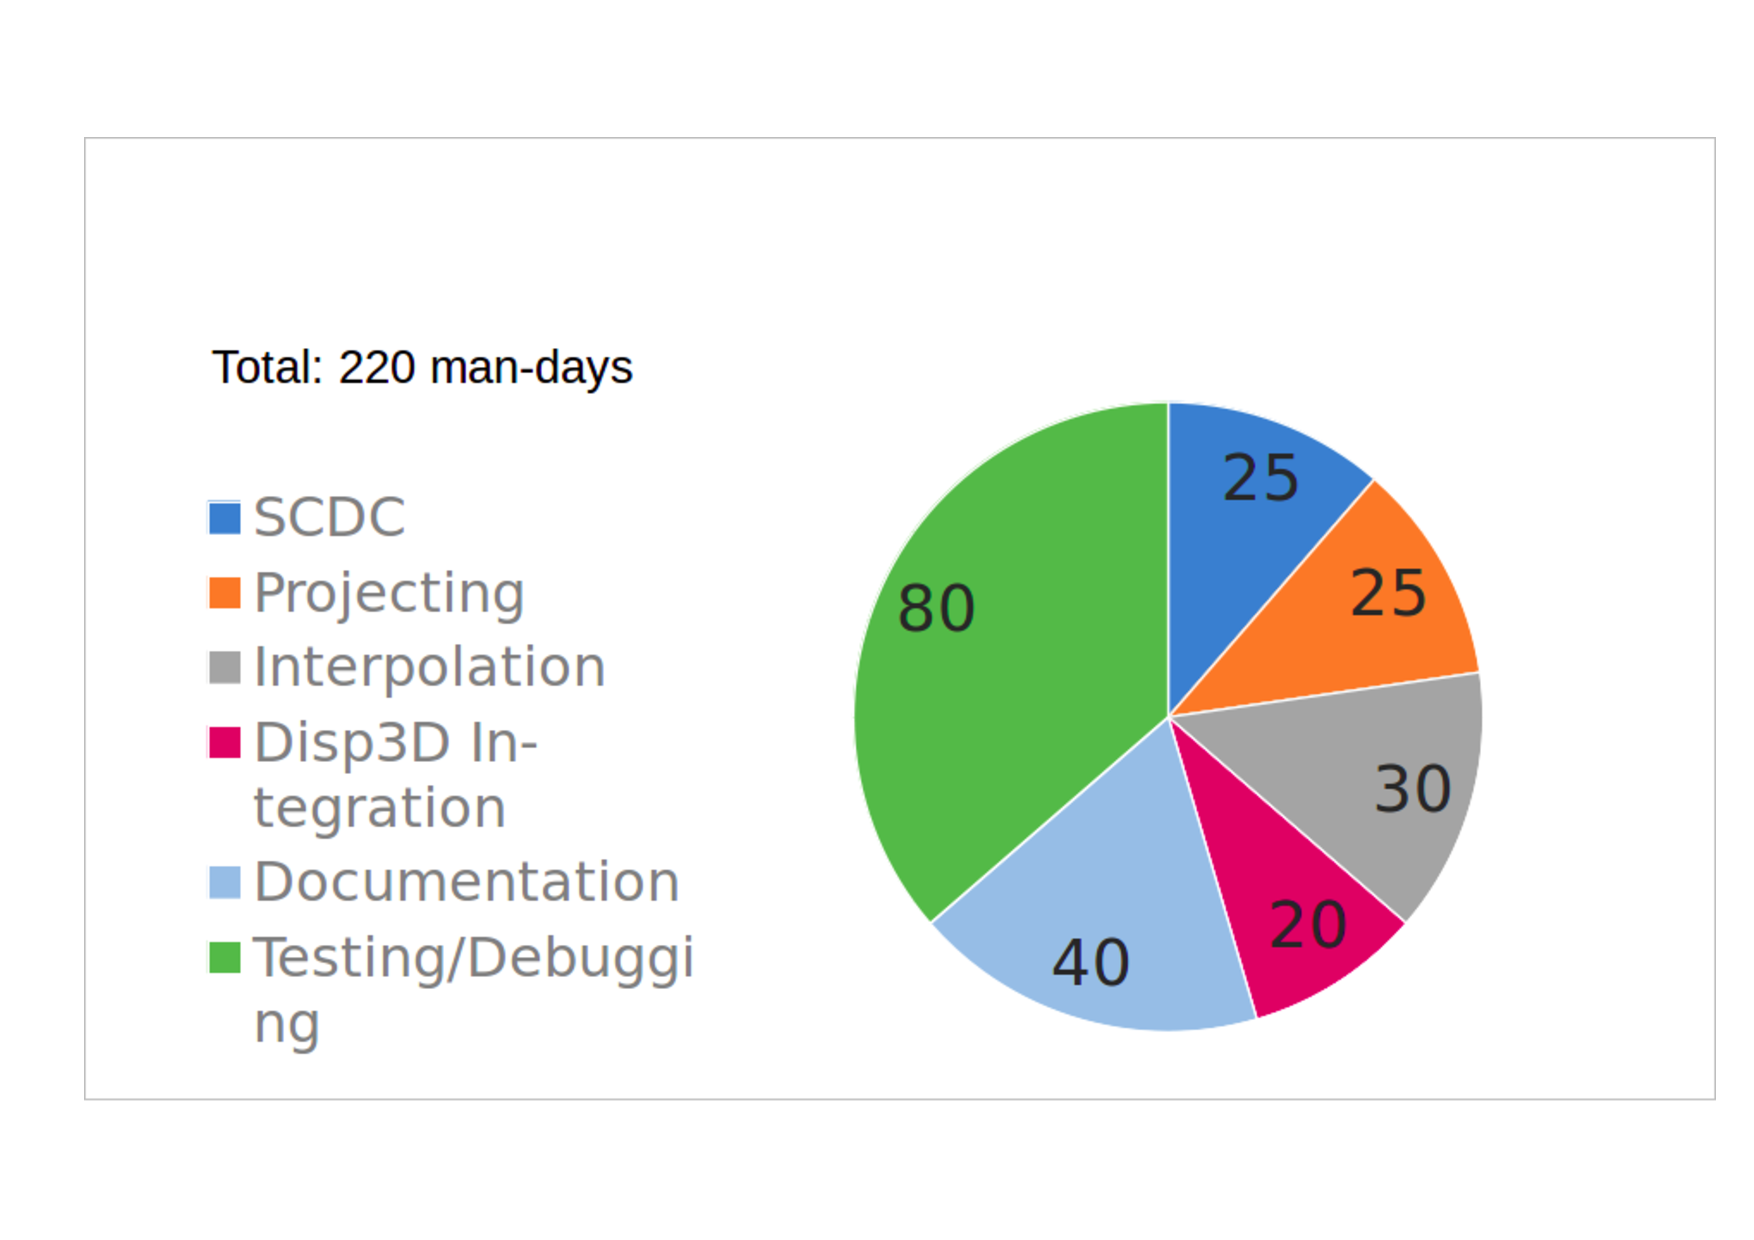
\includegraphics[width= 10cm]{figures/Aufwandsabschaetzung.pdf}
		\caption{Aufwandsabschätzung}
	\end{center}
\end{figure}

\subsection{Risk Estimation RE}
In this section, the probability of the different occurring risks involved in the Project is mentioned. If any risks take place, their effect helps determining how important it is for the team to take care of that risk and prevent it from happening again.

\begin{figure}
	\begin{center}
		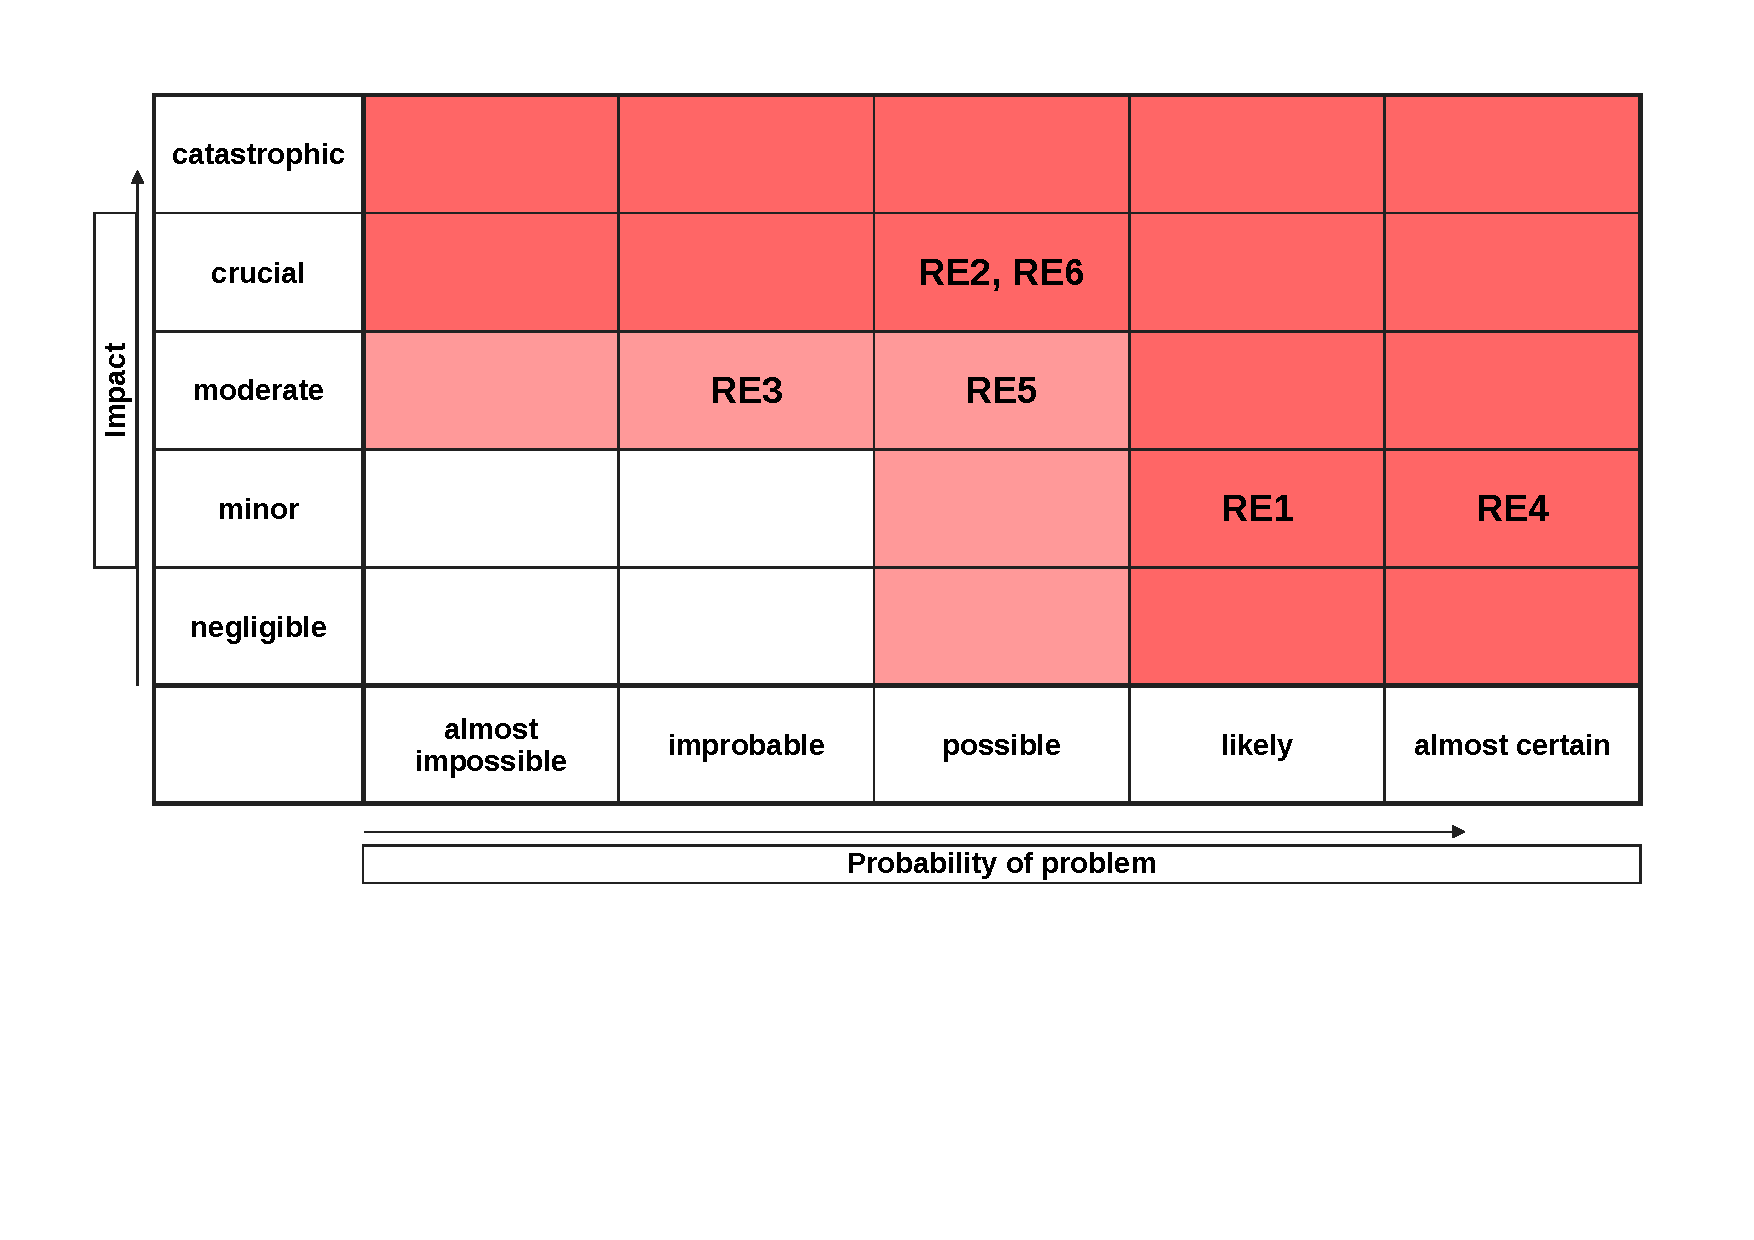
\includegraphics[width= 17cm]{figures/Risikoabschaetzung.pdf}
		\caption{Risk Estimation RE}
	\end{center}
\end{figure}


\begin{description}
	\item[RE1:] Communication problems in the team
	\item[RE2:] Coverage is too extensive
	\item[RE3:] Framework does not provide the needed functionality 
	\item[RE4:] Absence of the team members 
	\item[RE5:] Change of the requirements due to the miscommunication with the Product Owner PO
	\item[RE6:] Hidden complexity 
 \end{description}

\clearpage

\subsection{Milestones}
\begin{description}
	\leftskip=0,8cm
	\item[First Milestone:] functional specification, preliminary design, Reviewdocument, executable inputprocessing, Presentation 
	
	\item[Second Milestone:] SCDC (running), Projecting (running), Interpolation (running), Intergration display 3D, Reviewdocument, Presentation, detailed design
	
	\item[Third Milenstone:] Portation to MNE Scan, SCDC (tested and operating), Projecting (tested and operating), Interpolation (tested and operating), Reviewdocment, Presentation
\end{description}



\subsection{Organization}

This section concerns to the rules, agreements and the partitioning regarding the teamwork in the Project, so the work itself will at it best be efficient and organized. 

\subsubsection{Ways of communication}
\begin{description}
	\item[Telegram:] Used for quicker and direct team communication so that the possible misunderstandings will be solved in no time.
	
	\item[e-mail distribution list:] Used for scheduling the team meetings and the communications with the extended team, including the POs. 
	
	\item[Team meetings:] Used for the review and direct discussion of the encountered problems. 
	
	\item[Skype:] Used in the cases of the absence of a team member. 
	
	\item [Jira:] Used for scheduling tasks and keeping track of the progress done by each member of the team.
	
	\item[Dropbox:] Used for exchanging documents and file sharing.  
\end{description}

\subsubsection{Additional agreements}
\begin{itemize}
	\item Internal team meetings (without the POs) : (every week) Tuesdays and Thursdays at 19:00
	
	\item External team meeting (with the POs) : (every week) Wednesdays at 17:00
	
	\item Meeting of the subgroups : upon consultation and demand 
\end{itemize}

\subsubsection{Role assignment in Scrum}

\begin{description}
	\leftskip=0,8cm
	\item[Produkt Owner:] Thomas Jochmann, Lorenz Esch
	
	\item[Scrum Master:] Simon Heinke
	
	\item[Development team:] Blerta Hamzallari, Felix Griesau, Julius Lerm, Lars Debor, Marco Klamke, Simon Heinke, Sugandha Sachdeva, Petros Simidyan
	
	\item[Client, User:] Participants of the MNE CPP Project of Boston Child Hospital
	
\end{description}

\subsubsection{Role assignment organization}
\begin{description}
	\leftskip=0,8cm
	\item[Adviser:] Thomas Jochmann, Lorenz Esch
	
	\item[Team leader:] Simon Heinke
	
	\item[Code:] Lars Debor
	
	\item[Version Management :] Felix Griesau
	
\end{description}



\clearpage